\documentclass[12pt]{article}
\usepackage[margin=1in]{geometry} 
\usepackage{amsmath,amsthm,amssymb,amsfonts}
\usepackage{graphicx}
\usepackage{listings}
\usepackage{enumitem}
\usepackage{amsmath}
\usepackage{tikz}
\usepackage{stmaryrd}

\newcommand{\N}{\mathbb{N}}
\newcommand{\Z}{\mathbb{Z}}
 
\newenvironment{problem}[2][Problem]{\begin{trivlist}
\item[\hskip \labelsep {\bfseries #1}\hskip \labelsep {\bfseries #2.}]}{\end{trivlist}}
\setlength{\parskip}{1em}

\begin{document}
\title{COMP.3040 Homework 1}

\maketitle

\begin{problem}{2.1}
\end{problem}
\begin{enumerate}
	\item[(a)]~

		\tikzset{every picture/.style={line width=0.75pt}} %set default line width to 0.75pt        
		
		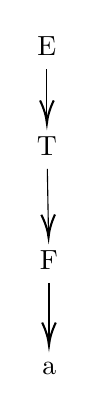
\begin{tikzpicture}[x=0.75pt,y=0.75pt,yscale=-1,xscale=1]
		%uncomment if require: \path (0,266.5); %set diagram left start at 0, and has height of 266.5
		
		% Text Node
		\draw (311,45) node  [align=left] {E};
		% Text Node
		\draw (311,93) node  [align=left] {T};
		% Text Node
		\draw (312,148) node  [align=left] {F};
		% Text Node
		\draw (312,200) node  [align=left] {a};
		% Connection
		\draw    (311,56) -- (311,80) ;
		\draw [shift={(311,82)}, rotate = 270] [color={rgb, 255:red, 0; green, 0; blue, 0 }  ][line width=0.75]    (10.93,-3.29) .. controls (6.95,-1.4) and (3.31,-0.3) .. (0,0) .. controls (3.31,0.3) and (6.95,1.4) .. (10.93,3.29)   ;
		
		% Connection
		\draw    (311.2,104) -- (311.76,135) ;
		\draw [shift={(311.8,137)}, rotate = 268.96] [color={rgb, 255:red, 0; green, 0; blue, 0 }  ][line width=0.75]    (10.93,-3.29) .. controls (6.95,-1.4) and (3.31,-0.3) .. (0,0) .. controls (3.31,0.3) and (6.95,1.4) .. (10.93,3.29)   ;
		
		% Connection
		\draw    (312,159) -- (312,187) ;
		\draw [shift={(312,189)}, rotate = 270] [color={rgb, 255:red, 0; green, 0; blue, 0 }  ][line width=0.75]    (10.93,-3.29) .. controls (6.95,-1.4) and (3.31,-0.3) .. (0,0) .. controls (3.31,0.3) and (6.95,1.4) .. (10.93,3.29)   ;
		
		\end{tikzpicture}

	\item[(b)]~

		\tikzset{every picture/.style={line width=0.75pt}} %set default line width to 0.75pt        
		
		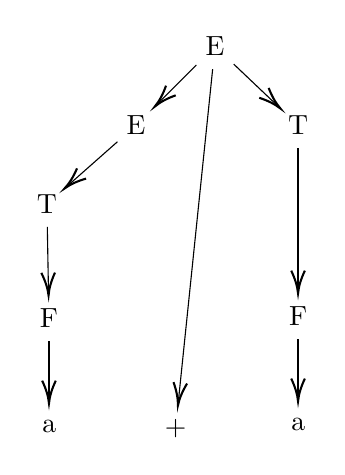
\begin{tikzpicture}[x=0.75pt,y=0.75pt,yscale=-1,xscale=1]
		%uncomment if require: \path (0,291); %set diagram left start at 0, and has height of 291
		
		% Text Node
		\draw (298,57) node  [align=left] {E};
		% Text Node
		\draw (338,95) node  [align=left] {T};
		% Text Node
		\draw (260,95) node  [align=left] {E};
		% Text Node
		\draw (217,133) node  [align=left] {T};
		% Text Node
		\draw (218,188) node  [align=left] {F};
		% Text Node
		\draw (218,240) node  [align=left] {a};
		% Text Node
		\draw (338,187) node  [align=left] {F};
		% Text Node
		\draw (338,239) node  [align=left] {a};
		% Text Node
		\draw (279,241) node  [align=left] {+};
		% Connection
		\draw    (307,65.55) -- (328.05,85.55) ;
		\draw [shift={(329.5,86.93)}, rotate = 223.53] [color={rgb, 255:red, 0; green, 0; blue, 0 }  ][line width=0.75]    (10.93,-3.29) .. controls (6.95,-1.4) and (3.31,-0.3) .. (0,0) .. controls (3.31,0.3) and (6.95,1.4) .. (10.93,3.29)   ;
		
		% Connection
		\draw    (289,66) -- (270.41,84.59) ;
		\draw [shift={(269,86)}, rotate = 315] [color={rgb, 255:red, 0; green, 0; blue, 0 }  ][line width=0.75]    (10.93,-3.29) .. controls (6.95,-1.4) and (3.31,-0.3) .. (0,0) .. controls (3.31,0.3) and (6.95,1.4) .. (10.93,3.29)   ;
		
		% Connection
		\draw    (217.2,144) -- (217.76,175) ;
		\draw [shift={(217.8,177)}, rotate = 268.96] [color={rgb, 255:red, 0; green, 0; blue, 0 }  ][line width=0.75]    (10.93,-3.29) .. controls (6.95,-1.4) and (3.31,-0.3) .. (0,0) .. controls (3.31,0.3) and (6.95,1.4) .. (10.93,3.29)   ;
		
		% Connection
		\draw    (218,199) -- (218,227) ;
		\draw [shift={(218,229)}, rotate = 270] [color={rgb, 255:red, 0; green, 0; blue, 0 }  ][line width=0.75]    (10.93,-3.29) .. controls (6.95,-1.4) and (3.31,-0.3) .. (0,0) .. controls (3.31,0.3) and (6.95,1.4) .. (10.93,3.29)   ;
		
		% Connection
		\draw    (251,102.95) -- (227,124.16) ;
		\draw [shift={(225.5,125.49)}, rotate = 318.53] [color={rgb, 255:red, 0; green, 0; blue, 0 }  ][line width=0.75]    (10.93,-3.29) .. controls (6.95,-1.4) and (3.31,-0.3) .. (0,0) .. controls (3.31,0.3) and (6.95,1.4) .. (10.93,3.29)   ;
		
		% Connection
		\draw    (338,198) -- (338,226) ;
		\draw [shift={(338,228)}, rotate = 270] [color={rgb, 255:red, 0; green, 0; blue, 0 }  ][line width=0.75]    (10.93,-3.29) .. controls (6.95,-1.4) and (3.31,-0.3) .. (0,0) .. controls (3.31,0.3) and (6.95,1.4) .. (10.93,3.29)   ;
		
		% Connection
		\draw    (338,106) -- (338,174) ;
		\draw [shift={(338,176)}, rotate = 270] [color={rgb, 255:red, 0; green, 0; blue, 0 }  ][line width=0.75]    (10.93,-3.29) .. controls (6.95,-1.4) and (3.31,-0.3) .. (0,0) .. controls (3.31,0.3) and (6.95,1.4) .. (10.93,3.29)   ;
		
		% Connection
		\draw    (296.86,68) -- (280.34,228.01) ;
		\draw [shift={(280.14,230)}, rotate = 275.9] [color={rgb, 255:red, 0; green, 0; blue, 0 }  ][line width=0.75]    (10.93,-3.29) .. controls (6.95,-1.4) and (3.31,-0.3) .. (0,0) .. controls (3.31,0.3) and (6.95,1.4) .. (10.93,3.29)   ;
		
		\end{tikzpicture}

	\item[(c)]~

		\tikzset{every picture/.style={line width=0.75pt}} %set default line width to 0.75pt        
		
		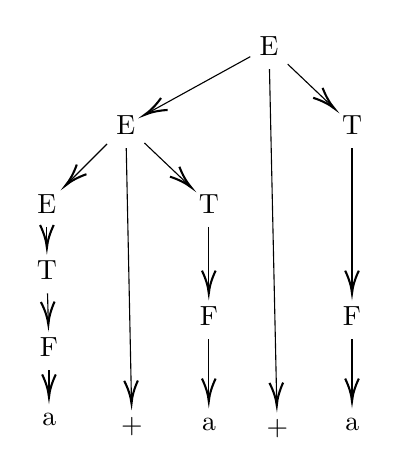
\begin{tikzpicture}[x=0.75pt,y=0.75pt,yscale=-1,xscale=1]
		%uncomment if require: \path (0,291); %set diagram left start at 0, and has height of 291
		
		% Text Node
		\draw (298,57) node  [align=left] {E};
		% Text Node
		\draw (338,95) node  [align=left] {T};
		% Text Node
		\draw (338,187) node  [align=left] {F};
		% Text Node
		\draw (338,239) node  [align=left] {a};
		% Text Node
		\draw (302,241) node  [align=left] {+};
		% Text Node
		\draw (191,165) node  [align=left] {T};
		% Text Node
		\draw (192,202) node  [align=left] {F};
		% Text Node
		\draw (192,237) node  [align=left] {a};
		% Text Node
		\draw (229,95) node  [align=left] {E};
		% Text Node
		\draw (269,133) node  [align=left] {T};
		% Text Node
		\draw (191,133) node  [align=left] {E};
		% Text Node
		\draw (269,187) node  [align=left] {F};
		% Text Node
		\draw (269,239) node  [align=left] {a};
		% Text Node
		\draw (232,240) node  [align=left] {+};
		% Connection
		\draw    (307,65.55) -- (328.05,85.55) ;
		\draw [shift={(329.5,86.93)}, rotate = 223.53] [color={rgb, 255:red, 0; green, 0; blue, 0 }  ][line width=0.75]    (10.93,-3.29) .. controls (6.95,-1.4) and (3.31,-0.3) .. (0,0) .. controls (3.31,0.3) and (6.95,1.4) .. (10.93,3.29)   ;
		
		% Connection
		\draw    (338,198) -- (338,226) ;
		\draw [shift={(338,228)}, rotate = 270] [color={rgb, 255:red, 0; green, 0; blue, 0 }  ][line width=0.75]    (10.93,-3.29) .. controls (6.95,-1.4) and (3.31,-0.3) .. (0,0) .. controls (3.31,0.3) and (6.95,1.4) .. (10.93,3.29)   ;
		
		% Connection
		\draw    (338,106) -- (338,174) ;
		\draw [shift={(338,176)}, rotate = 270] [color={rgb, 255:red, 0; green, 0; blue, 0 }  ][line width=0.75]    (10.93,-3.29) .. controls (6.95,-1.4) and (3.31,-0.3) .. (0,0) .. controls (3.31,0.3) and (6.95,1.4) .. (10.93,3.29)   ;
		
		% Connection
		\draw    (298.24,68) -- (301.72,228) ;
		\draw [shift={(301.76,230)}, rotate = 268.75] [color={rgb, 255:red, 0; green, 0; blue, 0 }  ][line width=0.75]    (10.93,-3.29) .. controls (6.95,-1.4) and (3.31,-0.3) .. (0,0) .. controls (3.31,0.3) and (6.95,1.4) .. (10.93,3.29)   ;
		
		% Connection
		\draw    (191.3,176) -- (191.65,189) ;
		\draw [shift={(191.7,191)}, rotate = 268.45] [color={rgb, 255:red, 0; green, 0; blue, 0 }  ][line width=0.75]    (10.93,-3.29) .. controls (6.95,-1.4) and (3.31,-0.3) .. (0,0) .. controls (3.31,0.3) and (6.95,1.4) .. (10.93,3.29)   ;
		
		% Connection
		\draw    (192,213) -- (192,224) ;
		\draw [shift={(192,226)}, rotate = 270] [color={rgb, 255:red, 0; green, 0; blue, 0 }  ][line width=0.75]    (10.93,-3.29) .. controls (6.95,-1.4) and (3.31,-0.3) .. (0,0) .. controls (3.31,0.3) and (6.95,1.4) .. (10.93,3.29)   ;
		
		% Connection
		\draw    (238,103.55) -- (259.05,123.55) ;
		\draw [shift={(260.5,124.93)}, rotate = 223.53] [color={rgb, 255:red, 0; green, 0; blue, 0 }  ][line width=0.75]    (10.93,-3.29) .. controls (6.95,-1.4) and (3.31,-0.3) .. (0,0) .. controls (3.31,0.3) and (6.95,1.4) .. (10.93,3.29)   ;
		
		% Connection
		\draw    (220,104) -- (201.41,122.59) ;
		\draw [shift={(200,124)}, rotate = 315] [color={rgb, 255:red, 0; green, 0; blue, 0 }  ][line width=0.75]    (10.93,-3.29) .. controls (6.95,-1.4) and (3.31,-0.3) .. (0,0) .. controls (3.31,0.3) and (6.95,1.4) .. (10.93,3.29)   ;
		
		% Connection
		\draw    (289,61.96) -- (239.75,89.08) ;
		\draw [shift={(238,90.04)}, rotate = 331.15999999999997] [color={rgb, 255:red, 0; green, 0; blue, 0 }  ][line width=0.75]    (10.93,-3.29) .. controls (6.95,-1.4) and (3.31,-0.3) .. (0,0) .. controls (3.31,0.3) and (6.95,1.4) .. (10.93,3.29)   ;
		
		% Connection
		\draw    (269,198) -- (269,226) ;
		\draw [shift={(269,228)}, rotate = 270] [color={rgb, 255:red, 0; green, 0; blue, 0 }  ][line width=0.75]    (10.93,-3.29) .. controls (6.95,-1.4) and (3.31,-0.3) .. (0,0) .. controls (3.31,0.3) and (6.95,1.4) .. (10.93,3.29)   ;
		
		% Connection
		\draw    (269,144) -- (269,174) ;
		\draw [shift={(269,176)}, rotate = 270] [color={rgb, 255:red, 0; green, 0; blue, 0 }  ][line width=0.75]    (10.93,-3.29) .. controls (6.95,-1.4) and (3.31,-0.3) .. (0,0) .. controls (3.31,0.3) and (6.95,1.4) .. (10.93,3.29)   ;
		
		% Connection
		\draw    (191,144) -- (191,152) ;
		\draw [shift={(191,154)}, rotate = 270] [color={rgb, 255:red, 0; green, 0; blue, 0 }  ][line width=0.75]    (10.93,-3.29) .. controls (6.95,-1.4) and (3.31,-0.3) .. (0,0) .. controls (3.31,0.3) and (6.95,1.4) .. (10.93,3.29)   ;
		
		% Connection
		\draw    (229.23,106) -- (231.73,227) ;
		\draw [shift={(231.77,229)}, rotate = 268.81] [color={rgb, 255:red, 0; green, 0; blue, 0 }  ][line width=0.75]    (10.93,-3.29) .. controls (6.95,-1.4) and (3.31,-0.3) .. (0,0) .. controls (3.31,0.3) and (6.95,1.4) .. (10.93,3.29)   ;
		
		\end{tikzpicture}

	\item[(d)]

		\tikzset{every picture/.style={line width=0.75pt}} %set default line width to 0.75pt        
		
		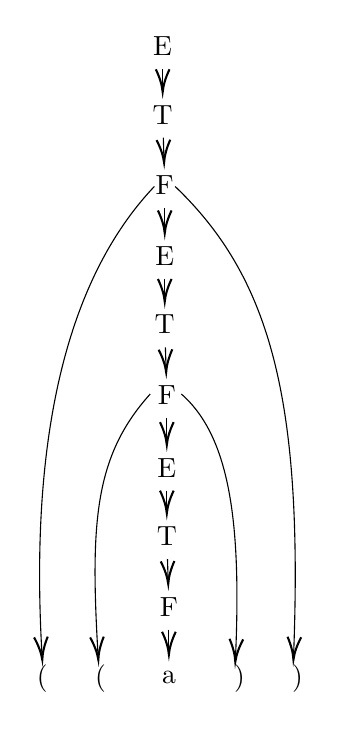
\begin{tikzpicture}[x=0.75pt,y=0.75pt,yscale=-1,xscale=1]
		%uncomment if require: \path (0,409.5); %set diagram left start at 0, and has height of 409.5
		
		%Curve Lines [id:da8633373547677052] 
		\draw    (342,107.5) .. controls (286.56,165.91) and (284.05,267.44) .. (287.88,333.51) ;
		\draw [shift={(288,335.5)}, rotate = 266.53] [color={rgb, 255:red, 0; green, 0; blue, 0 }  ][line width=0.75]    (10.93,-3.29) .. controls (6.95,-1.4) and (3.31,-0.3) .. (0,0) .. controls (3.31,0.3) and (6.95,1.4) .. (10.93,3.29)   ;
		
		%Curve Lines [id:da7557276714024137] 
		\draw    (340,207.5) .. controls (313.27,237.2) and (311.04,268.86) .. (314.88,333.53) ;
		\draw [shift={(315,335.5)}, rotate = 266.53] [color={rgb, 255:red, 0; green, 0; blue, 0 }  ][line width=0.75]    (10.93,-3.29) .. controls (6.95,-1.4) and (3.31,-0.3) .. (0,0) .. controls (3.31,0.3) and (6.95,1.4) .. (10.93,3.29)   ;
		
		%Curve Lines [id:da46852940249148056] 
		\draw    (352,107.5) .. controls (397.77,151.28) and (413.84,209.91) .. (409.07,333.63) ;
		\draw [shift={(409,335.5)}, rotate = 272.29] [color={rgb, 255:red, 0; green, 0; blue, 0 }  ][line width=0.75]    (10.93,-3.29) .. controls (6.95,-1.4) and (3.31,-0.3) .. (0,0) .. controls (3.31,0.3) and (6.95,1.4) .. (10.93,3.29)   ;
		
		%Curve Lines [id:da5180551817069581] 
		\draw    (355,207.5) .. controls (378.76,228.29) and (383.9,270.64) .. (381.09,334.56) ;
		\draw [shift={(381,336.5)}, rotate = 272.64] [color={rgb, 255:red, 0; green, 0; blue, 0 }  ][line width=0.75]    (10.93,-3.29) .. controls (6.95,-1.4) and (3.31,-0.3) .. (0,0) .. controls (3.31,0.3) and (6.95,1.4) .. (10.93,3.29)   ;
		
		% Text Node
		\draw (346,40) node  [align=left] {E};
		% Text Node
		\draw (346,73) node  [align=left] {T};
		% Text Node
		\draw (347,107) node  [align=left] {F};
		% Text Node
		\draw (347,141) node  [align=left] {E};
		% Text Node
		\draw (347,174) node  [align=left] {T};
		% Text Node
		\draw (348,208) node  [align=left] {F};
		% Text Node
		\draw (348,243) node  [align=left] {E};
		% Text Node
		\draw (348,276) node  [align=left] {T};
		% Text Node
		\draw (349,310) node  [align=left] {F};
		% Text Node
		\draw (349,344) node  [align=left] {a};
		% Text Node
		\draw (316,344.5) node  [align=left] {(};
		% Text Node
		\draw (383,344.5) node  [align=left] {)};
		% Text Node
		\draw (288,344.5) node  [align=left] {(};
		% Text Node
		\draw (411,344.5) node  [align=left] {)};
		% Connection
		\draw    (346,51) -- (346,60) ;
		\draw [shift={(346,62)}, rotate = 270] [color={rgb, 255:red, 0; green, 0; blue, 0 }  ][line width=0.75]    (10.93,-3.29) .. controls (6.95,-1.4) and (3.31,-0.3) .. (0,0) .. controls (3.31,0.3) and (6.95,1.4) .. (10.93,3.29)   ;
		
		% Connection
		\draw    (346.32,84) -- (346.62,94) ;
		\draw [shift={(346.68,96)}, rotate = 268.32] [color={rgb, 255:red, 0; green, 0; blue, 0 }  ][line width=0.75]    (10.93,-3.29) .. controls (6.95,-1.4) and (3.31,-0.3) .. (0,0) .. controls (3.31,0.3) and (6.95,1.4) .. (10.93,3.29)   ;
		
		% Connection
		\draw    (347,152) -- (347,161) ;
		\draw [shift={(347,163)}, rotate = 270] [color={rgb, 255:red, 0; green, 0; blue, 0 }  ][line width=0.75]    (10.93,-3.29) .. controls (6.95,-1.4) and (3.31,-0.3) .. (0,0) .. controls (3.31,0.3) and (6.95,1.4) .. (10.93,3.29)   ;
		
		% Connection
		\draw    (347.32,185) -- (347.62,195) ;
		\draw [shift={(347.68,197)}, rotate = 268.32] [color={rgb, 255:red, 0; green, 0; blue, 0 }  ][line width=0.75]    (10.93,-3.29) .. controls (6.95,-1.4) and (3.31,-0.3) .. (0,0) .. controls (3.31,0.3) and (6.95,1.4) .. (10.93,3.29)   ;
		
		% Connection
		\draw    (348,254) -- (348,263) ;
		\draw [shift={(348,265)}, rotate = 270] [color={rgb, 255:red, 0; green, 0; blue, 0 }  ][line width=0.75]    (10.93,-3.29) .. controls (6.95,-1.4) and (3.31,-0.3) .. (0,0) .. controls (3.31,0.3) and (6.95,1.4) .. (10.93,3.29)   ;
		
		% Connection
		\draw    (348.32,287) -- (348.62,297) ;
		\draw [shift={(348.68,299)}, rotate = 268.32] [color={rgb, 255:red, 0; green, 0; blue, 0 }  ][line width=0.75]    (10.93,-3.29) .. controls (6.95,-1.4) and (3.31,-0.3) .. (0,0) .. controls (3.31,0.3) and (6.95,1.4) .. (10.93,3.29)   ;
		
		% Connection
		\draw    (347,118) -- (347,128) ;
		\draw [shift={(347,130)}, rotate = 270] [color={rgb, 255:red, 0; green, 0; blue, 0 }  ][line width=0.75]    (10.93,-3.29) .. controls (6.95,-1.4) and (3.31,-0.3) .. (0,0) .. controls (3.31,0.3) and (6.95,1.4) .. (10.93,3.29)   ;
		
		% Connection
		\draw    (348,219) -- (348,230) ;
		\draw [shift={(348,232)}, rotate = 270] [color={rgb, 255:red, 0; green, 0; blue, 0 }  ][line width=0.75]    (10.93,-3.29) .. controls (6.95,-1.4) and (3.31,-0.3) .. (0,0) .. controls (3.31,0.3) and (6.95,1.4) .. (10.93,3.29)   ;
		
		% Connection
		\draw    (349,321) -- (349,331) ;
		\draw [shift={(349,333)}, rotate = 270] [color={rgb, 255:red, 0; green, 0; blue, 0 }  ][line width=0.75]    (10.93,-3.29) .. controls (6.95,-1.4) and (3.31,-0.3) .. (0,0) .. controls (3.31,0.3) and (6.95,1.4) .. (10.93,3.29)   ;
		
		\end{tikzpicture}

\end{enumerate}

\begin{problem}{2.4}
\end{problem}
\begin{enumerate}
	\item[(b)]
			$G_b$ = ($\{S, S_0\}, \{0,1\}, R, S$)	\\
			R: 	\\
				$S \to 0S_00 \: | \: 1S_01$	\\
				$S_0 \to 0S_0 \: | \: 1S_0 \: | \: 0 \: | \: 1$

	\item[(c)]
			$G_c$ = ($\{S, S_0\}, \{0,1\}, R, S$)	\\
			R: 	\\
				$S \to 0S_0 \: | \: 1S_0$	\\
				$S_0 \to 00S_0 \: | \: 01S_0 \: | \: 10S_0 \: | \: 11S_0 \: | \: 00 \: | \: 01 \: | \: 10 \: | \: 11$
	\item[(e)]
			$G_e$ = ($\{S\}, \{0,1\}, R, S$)	\\
			R: 	\\
				$S \to 0S0 \: | \: 1S1 \: | \: 1 \: | \: 0 \: | \: 00 \: | \: 11$
	\item[(f)]
			$G_b$ = ($\{S\}, \{0,1\}, R, S$)	\\
			R: 	\\
				$S \to S$
\end{enumerate}

\begin{problem}{2.5}
\end{problem}
\begin{enumerate}
	\item[(b)]
		1. Read first input and push to stack. 	\\
		2. Skip all following input till reads the last input. If last input equals to symbol at top of stack, accept input. 

		\tikzset{every picture/.style={line width=0.75pt}} %set default line width to 0.75pt        
		
		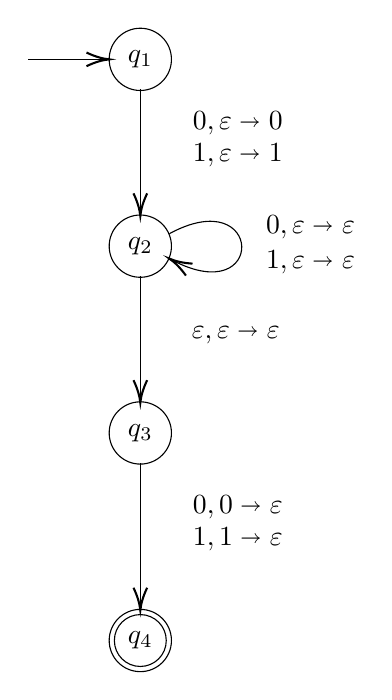
\begin{tikzpicture}[x=0.75pt,y=0.75pt,yscale=-1,xscale=1]
		%uncomment if require: \path (0,352); %set diagram left start at 0, and has height of 352
		
		%Shape: Circle [id:dp12453177844053687] 
		\draw   (279,30.85) .. controls (279,22.56) and (285.72,15.85) .. (294,15.85) .. controls (302.28,15.85) and (309,22.56) .. (309,30.85) .. controls (309,39.13) and (302.28,45.85) .. (294,45.85) .. controls (285.72,45.85) and (279,39.13) .. (279,30.85) -- cycle ;
		%Straight Lines [id:da41507407708092514] 
		\draw    (240,30.85) -- (277,30.85) ;
		\draw [shift={(279,30.85)}, rotate = 180] [color={rgb, 255:red, 0; green, 0; blue, 0 }  ][line width=0.75]    (10.93,-3.29) .. controls (6.95,-1.4) and (3.31,-0.3) .. (0,0) .. controls (3.31,0.3) and (6.95,1.4) .. (10.93,3.29)   ;
		
		%Shape: Circle [id:dp1864135168005152] 
		\draw   (279,120.85) .. controls (279,112.56) and (285.72,105.85) .. (294,105.85) .. controls (302.28,105.85) and (309,112.56) .. (309,120.85) .. controls (309,129.13) and (302.28,135.85) .. (294,135.85) .. controls (285.72,135.85) and (279,129.13) .. (279,120.85) -- cycle ;
		%Shape: Circle [id:dp47653412527109396] 
		\draw   (279,210.85) .. controls (279,202.56) and (285.72,195.85) .. (294,195.85) .. controls (302.28,195.85) and (309,202.56) .. (309,210.85) .. controls (309,219.13) and (302.28,225.85) .. (294,225.85) .. controls (285.72,225.85) and (279,219.13) .. (279,210.85) -- cycle ;
		%Curve Lines [id:da5909762327175239] 
		\draw    (308,114.85) .. controls (353.54,90.1) and (354.98,151.6) .. (309.4,127.6) ;
		\draw [shift={(308,126.85)}, rotate = 388.95] [color={rgb, 255:red, 0; green, 0; blue, 0 }  ][line width=0.75]    (10.93,-3.29) .. controls (6.95,-1.4) and (3.31,-0.3) .. (0,0) .. controls (3.31,0.3) and (6.95,1.4) .. (10.93,3.29)   ;
		
		%Shape: Circle [id:dp5425726544476028] 
		\draw   (281.5,310.85) .. controls (281.5,303.94) and (287.1,298.35) .. (294,298.35) .. controls (300.9,298.35) and (306.5,303.94) .. (306.5,310.85) .. controls (306.5,317.75) and (300.9,323.35) .. (294,323.35) .. controls (287.1,323.35) and (281.5,317.75) .. (281.5,310.85) -- cycle ;
		%Shape: Circle [id:dp5908513707780341] 
		\draw   (279,310.85) .. controls (279,302.56) and (285.72,295.85) .. (294,295.85) .. controls (302.28,295.85) and (309,302.56) .. (309,310.85) .. controls (309,319.13) and (302.28,325.85) .. (294,325.85) .. controls (285.72,325.85) and (279,319.13) .. (279,310.85) -- cycle ;
		
		% Text Node
		\draw (294,30.85) node  [align=left] {$\displaystyle q_{1}$};
		% Text Node
		\draw (294,120.85) node  [align=left] {$\displaystyle q_{2}$};
		% Text Node
		\draw (294,210.85) node  [align=left] {$\displaystyle q_{3}$};
		% Text Node
		\draw (341,76.85) node  [align=left] {$\displaystyle {\textstyle 1,\varepsilon \shortrightarrow 1}$};
		% Text Node
		\draw (341,61.85) node  [align=left] {$\displaystyle {\textstyle 0,\varepsilon \shortrightarrow 0}$};
		% Text Node
		\draw (376,128.85) node  [align=left] {$\displaystyle 1,\varepsilon \shortrightarrow \varepsilon $};
		% Text Node
		\draw (376,111.85) node  [align=left] {$\displaystyle 0,\varepsilon \shortrightarrow \varepsilon $};
		% Text Node
		\draw (340,163.85) node  [align=left] {$\displaystyle \varepsilon ,\varepsilon \shortrightarrow \varepsilon $};
		% Text Node
		\draw (294,310.85) node  [align=left] {$\displaystyle q_{4}$};
		% Text Node
		\draw (341,261.85) node  [align=left] {$\displaystyle {\textstyle 1,1\shortrightarrow \varepsilon }$};
		% Text Node
		\draw (341,246.85) node  [align=left] {$\displaystyle {\textstyle 0,0\shortrightarrow \varepsilon }$};
		% Connection
		\draw    (294,45.35) -- (294,104.35) ;
		\draw [shift={(294,106.35)}, rotate = 270] [color={rgb, 255:red, 0; green, 0; blue, 0 }  ][line width=0.75]    (10.93,-3.29) .. controls (6.95,-1.4) and (3.31,-0.3) .. (0,0) .. controls (3.31,0.3) and (6.95,1.4) .. (10.93,3.29)   ;
		
		% Connection
		\draw    (294,135.35) -- (294,194.35) ;
		\draw [shift={(294,196.35)}, rotate = 270] [color={rgb, 255:red, 0; green, 0; blue, 0 }  ][line width=0.75]    (10.93,-3.29) .. controls (6.95,-1.4) and (3.31,-0.3) .. (0,0) .. controls (3.31,0.3) and (6.95,1.4) .. (10.93,3.29)   ;
		
		% Connection
		\draw    (294,225.35) -- (294,294.35) ;
		\draw [shift={(294,296.35)}, rotate = 270] [color={rgb, 255:red, 0; green, 0; blue, 0 }  ][line width=0.75]    (10.93,-3.29) .. controls (6.95,-1.4) and (3.31,-0.3) .. (0,0) .. controls (3.31,0.3) and (6.95,1.4) .. (10.93,3.29)   ;
		
		\end{tikzpicture}

	\item[(c)]
		1. Push 1 to stack. 	\\
		2. Read input. If number in stack is 1 accept input. Pop stack and push inverse symbol to stack. 	\\
		3. Repeat Step 2. 

		\tikzset{every picture/.style={line width=0.75pt}} %set default line width to 0.75pt        
		
		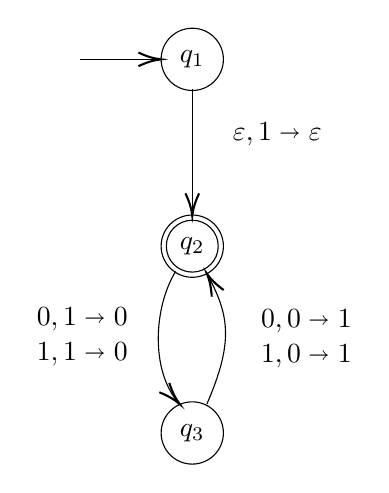
\begin{tikzpicture}[x=0.75pt,y=0.75pt,yscale=-1,xscale=1]
		%uncomment if require: \path (0,238); %set diagram left start at 0, and has height of 238
		
		%Shape: Circle [id:dp022800413258042607] 
		\draw   (310,28.85) .. controls (310,20.56) and (316.72,13.85) .. (325,13.85) .. controls (333.28,13.85) and (340,20.56) .. (340,28.85) .. controls (340,37.13) and (333.28,43.85) .. (325,43.85) .. controls (316.72,43.85) and (310,37.13) .. (310,28.85) -- cycle ;
		%Straight Lines [id:da42424073913097016] 
		\draw    (271,28.85) -- (308,28.85) ;
		\draw [shift={(310,28.85)}, rotate = 180] [color={rgb, 255:red, 0; green, 0; blue, 0 }  ][line width=0.75]    (10.93,-3.29) .. controls (6.95,-1.4) and (3.31,-0.3) .. (0,0) .. controls (3.31,0.3) and (6.95,1.4) .. (10.93,3.29)   ;
		
		%Shape: Circle [id:dp503642834669215] 
		\draw   (310,118.85) .. controls (310,110.56) and (316.72,103.85) .. (325,103.85) .. controls (333.28,103.85) and (340,110.56) .. (340,118.85) .. controls (340,127.13) and (333.28,133.85) .. (325,133.85) .. controls (316.72,133.85) and (310,127.13) .. (310,118.85) -- cycle ;
		%Shape: Circle [id:dp8194101144056025] 
		\draw   (310,208.85) .. controls (310,200.56) and (316.72,193.85) .. (325,193.85) .. controls (333.28,193.85) and (340,200.56) .. (340,208.85) .. controls (340,217.13) and (333.28,223.85) .. (325,223.85) .. controls (316.72,223.85) and (310,217.13) .. (310,208.85) -- cycle ;
		%Shape: Circle [id:dp6399295033492636] 
		\draw   (312.5,118.85) .. controls (312.5,111.94) and (318.1,106.35) .. (325,106.35) .. controls (331.9,106.35) and (337.5,111.94) .. (337.5,118.85) .. controls (337.5,125.75) and (331.9,131.35) .. (325,131.35) .. controls (318.1,131.35) and (312.5,125.75) .. (312.5,118.85) -- cycle ;
		%Curve Lines [id:da873998982192012] 
		\draw    (317,131) .. controls (306.33,148.46) and (305.07,178.15) .. (317.78,193.61) ;
		\draw [shift={(319,195)}, rotate = 226.97] [color={rgb, 255:red, 0; green, 0; blue, 0 }  ][line width=0.75]    (10.93,-3.29) .. controls (6.95,-1.4) and (3.31,-0.3) .. (0,0) .. controls (3.31,0.3) and (6.95,1.4) .. (10.93,3.29)   ;
		
		%Curve Lines [id:da9828990516588934] 
		\draw    (332.97,133.78) .. controls (343.11,152.8) and (344.61,165.9) .. (332,195) ;
		
		\draw [shift={(332,132)}, rotate = 61.19] [color={rgb, 255:red, 0; green, 0; blue, 0 }  ][line width=0.75]    (10.93,-3.29) .. controls (6.95,-1.4) and (3.31,-0.3) .. (0,0) .. controls (3.31,0.3) and (6.95,1.4) .. (10.93,3.29)   ;
		
		% Text Node
		\draw (325,28.85) node  [align=left] {$\displaystyle q_{1}$};
		% Text Node
		\draw (325,118.85) node  [align=left] {$\displaystyle q_{2}$};
		% Text Node
		\draw (325,208.85) node  [align=left] {$\displaystyle q_{3}$};
		% Text Node
		\draw (366,64.85) node  [align=left] {$\displaystyle {\textstyle \varepsilon ,1\shortrightarrow \varepsilon }$};
		% Text Node
		\draw (272,170.85) node  [align=left] {$\displaystyle 1,1\shortrightarrow 0$};
		% Text Node
		\draw (272,153.85) node  [align=left] {$\displaystyle 0,1\shortrightarrow 0$};
		% Text Node
		\draw (380,171.85) node  [align=left] {$\displaystyle 1,0\shortrightarrow 1$};
		% Text Node
		\draw (380,154.85) node  [align=left] {$\displaystyle 0,0\shortrightarrow 1$};
		% Connection
		\draw    (325,43.35) -- (325,102.35) ;
		\draw [shift={(325,104.35)}, rotate = 270] [color={rgb, 255:red, 0; green, 0; blue, 0 }  ][line width=0.75]    (10.93,-3.29) .. controls (6.95,-1.4) and (3.31,-0.3) .. (0,0) .. controls (3.31,0.3) and (6.95,1.4) .. (10.93,3.29)   ;
		
		\end{tikzpicture}

	\item[(e)]
		1. Keep reading input and push to stack. 	\\
		2. When reach to middle of string, if there is a center symbol, skip it. 	\\
		3. Read input and pop stack. If input does not equal to popped symbol or input is finished before, reject input. 	\\
		4. When empty stack and finish input, accept input. 

		\tikzset{every picture/.style={line width=0.75pt}} %set default line width to 0.75pt        
		
		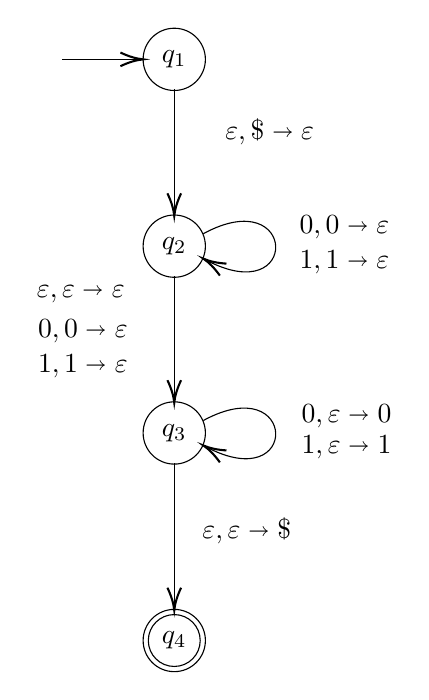
\begin{tikzpicture}[x=0.75pt,y=0.75pt,yscale=-1,xscale=1]
		%uncomment if require: \path (0,338.5); %set diagram left start at 0, and has height of 338.5
		
		%Shape: Circle [id:dp26907689339532537] 
		\draw   (288,27) .. controls (288,18.72) and (294.72,12) .. (303,12) .. controls (311.28,12) and (318,18.72) .. (318,27) .. controls (318,35.28) and (311.28,42) .. (303,42) .. controls (294.72,42) and (288,35.28) .. (288,27) -- cycle ;
		%Straight Lines [id:da11696011762706982] 
		\draw    (249,27) -- (286,27) ;
		\draw [shift={(288,27)}, rotate = 180] [color={rgb, 255:red, 0; green, 0; blue, 0 }  ][line width=0.75]    (10.93,-3.29) .. controls (6.95,-1.4) and (3.31,-0.3) .. (0,0) .. controls (3.31,0.3) and (6.95,1.4) .. (10.93,3.29)   ;
		
		%Shape: Circle [id:dp5529144800252732] 
		\draw   (288,117) .. controls (288,108.72) and (294.72,102) .. (303,102) .. controls (311.28,102) and (318,108.72) .. (318,117) .. controls (318,125.28) and (311.28,132) .. (303,132) .. controls (294.72,132) and (288,125.28) .. (288,117) -- cycle ;
		%Shape: Circle [id:dp7152024691115373] 
		\draw   (288,207) .. controls (288,198.72) and (294.72,192) .. (303,192) .. controls (311.28,192) and (318,198.72) .. (318,207) .. controls (318,215.28) and (311.28,222) .. (303,222) .. controls (294.72,222) and (288,215.28) .. (288,207) -- cycle ;
		%Curve Lines [id:da15247513241194155] 
		\draw    (317,111) .. controls (362.54,86.25) and (363.98,147.75) .. (318.4,123.75) ;
		\draw [shift={(317,123)}, rotate = 388.95] [color={rgb, 255:red, 0; green, 0; blue, 0 }  ][line width=0.75]    (10.93,-3.29) .. controls (6.95,-1.4) and (3.31,-0.3) .. (0,0) .. controls (3.31,0.3) and (6.95,1.4) .. (10.93,3.29)   ;
		
		%Shape: Circle [id:dp1809240273694217] 
		\draw   (290.5,307) .. controls (290.5,300.1) and (296.1,294.5) .. (303,294.5) .. controls (309.9,294.5) and (315.5,300.1) .. (315.5,307) .. controls (315.5,313.9) and (309.9,319.5) .. (303,319.5) .. controls (296.1,319.5) and (290.5,313.9) .. (290.5,307) -- cycle ;
		%Shape: Circle [id:dp6709419054009844] 
		\draw   (288,307) .. controls (288,298.72) and (294.72,292) .. (303,292) .. controls (311.28,292) and (318,298.72) .. (318,307) .. controls (318,315.28) and (311.28,322) .. (303,322) .. controls (294.72,322) and (288,315.28) .. (288,307) -- cycle ;
		%Curve Lines [id:da10390907640768199] 
		\draw    (317,201) .. controls (362.54,176.25) and (363.98,237.75) .. (318.4,213.75) ;
		\draw [shift={(317,213)}, rotate = 388.95] [color={rgb, 255:red, 0; green, 0; blue, 0 }  ][line width=0.75]    (10.93,-3.29) .. controls (6.95,-1.4) and (3.31,-0.3) .. (0,0) .. controls (3.31,0.3) and (6.95,1.4) .. (10.93,3.29)   ;
		
		% Text Node
		\draw (303,27) node  [align=left] {$\displaystyle q_{1}$};
		% Text Node
		\draw (303,117) node  [align=left] {$\displaystyle q_{2}$};
		% Text Node
		\draw (303,207) node  [align=left] {$\displaystyle q_{3}$};
		% Text Node
		\draw (349,62) node  [align=left] {$\displaystyle {\textstyle \varepsilon ,\$\shortrightarrow \varepsilon }$};
		% Text Node
		\draw (385,125) node  [align=left] {$\displaystyle 1,1\shortrightarrow \varepsilon $};
		% Text Node
		\draw (385,108) node  [align=left] {$\displaystyle 0,0\shortrightarrow \varepsilon $};
		% Text Node
		\draw (258,140) node  [align=left] {$\displaystyle \varepsilon ,\varepsilon \shortrightarrow \varepsilon $};
		% Text Node
		\draw (303,307) node  [align=left] {$\displaystyle q_{4}$};
		% Text Node
		\draw (386,214) node  [align=left] {$\displaystyle {\textstyle 1,\varepsilon \shortrightarrow 1}$};
		% Text Node
		\draw (386,199) node  [align=left] {$\displaystyle {\textstyle 0,\varepsilon \shortrightarrow 0}$};
		% Text Node
		\draw (259,175) node  [align=left] {$\displaystyle 1,1\shortrightarrow \varepsilon $};
		% Text Node
		\draw (259,158) node  [align=left] {$\displaystyle 0,0\shortrightarrow \varepsilon $};
		% Text Node
		\draw (338,254) node  [align=left] {$\displaystyle {\textstyle \varepsilon ,\varepsilon \shortrightarrow \$}$};
		% Connection
		\draw    (303,41.5) -- (303,100.5) ;
		\draw [shift={(303,102.5)}, rotate = 270] [color={rgb, 255:red, 0; green, 0; blue, 0 }  ][line width=0.75]    (10.93,-3.29) .. controls (6.95,-1.4) and (3.31,-0.3) .. (0,0) .. controls (3.31,0.3) and (6.95,1.4) .. (10.93,3.29)   ;
		
		% Connection
		\draw    (303,131.5) -- (303,190.5) ;
		\draw [shift={(303,192.5)}, rotate = 270] [color={rgb, 255:red, 0; green, 0; blue, 0 }  ][line width=0.75]    (10.93,-3.29) .. controls (6.95,-1.4) and (3.31,-0.3) .. (0,0) .. controls (3.31,0.3) and (6.95,1.4) .. (10.93,3.29)   ;
		
		% Connection
		\draw    (303,221.5) -- (303,290.5) ;
		\draw [shift={(303,292.5)}, rotate = 270] [color={rgb, 255:red, 0; green, 0; blue, 0 }  ][line width=0.75]    (10.93,-3.29) .. controls (6.95,-1.4) and (3.31,-0.3) .. (0,0) .. controls (3.31,0.3) and (6.95,1.4) .. (10.93,3.29)   ;
		
		\end{tikzpicture}

	\item[(f)]
		Ignore all input. 

		\tikzset{every picture/.style={line width=0.75pt}} %set default line width to 0.75pt        
		
		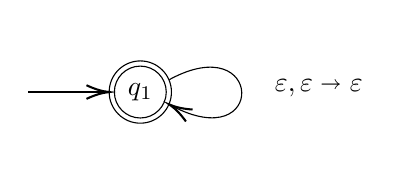
\begin{tikzpicture}[x=0.75pt,y=0.75pt,yscale=-1,xscale=1]
		%uncomment if require: \path (0,79); %set diagram left start at 0, and has height of 79
		
		%Shape: Circle [id:dp7506114950181269] 
		\draw   (288,35) .. controls (288,26.72) and (294.72,20) .. (303,20) .. controls (311.28,20) and (318,26.72) .. (318,35) .. controls (318,43.28) and (311.28,50) .. (303,50) .. controls (294.72,50) and (288,43.28) .. (288,35) -- cycle ;
		%Curve Lines [id:da4483416959061777] 
		\draw    (317,29) .. controls (362.54,4.25) and (363.98,65.75) .. (318.4,41.75) ;
		\draw [shift={(317,41)}, rotate = 388.95] [color={rgb, 255:red, 0; green, 0; blue, 0 }  ][line width=0.75]    (10.93,-3.29) .. controls (6.95,-1.4) and (3.31,-0.3) .. (0,0) .. controls (3.31,0.3) and (6.95,1.4) .. (10.93,3.29)   ;
		
		%Straight Lines [id:da38704998679010316] 
		\draw    (249,35) -- (286,35) ;
		\draw [shift={(288,35)}, rotate = 180] [color={rgb, 255:red, 0; green, 0; blue, 0 }  ][line width=0.75]    (10.93,-3.29) .. controls (6.95,-1.4) and (3.31,-0.3) .. (0,0) .. controls (3.31,0.3) and (6.95,1.4) .. (10.93,3.29)   ;
		
		%Shape: Circle [id:dp3065844361748524] 
		\draw   (290.5,35) .. controls (290.5,28.1) and (296.1,22.5) .. (303,22.5) .. controls (309.9,22.5) and (315.5,28.1) .. (315.5,35) .. controls (315.5,41.9) and (309.9,47.5) .. (303,47.5) .. controls (296.1,47.5) and (290.5,41.9) .. (290.5,35) -- cycle ;
		
		% Text Node
		\draw (303,35) node  [align=left] {$\displaystyle q_{1}$};
		% Text Node
		\draw (389,33) node  [align=left] {$\displaystyle {\textstyle \varepsilon ,\varepsilon \shortrightarrow \varepsilon }$};
		
		\end{tikzpicture}

\end{enumerate}

\begin{problem}{2.6}
\end{problem}
\begin{enumerate}
	\item[(b)]
		$G_b$ = ($\{S, S_a, S_{ab}, S_{aba}, S_b, S_{ba}, S_{bab}, S_x\}, \{a,b\}, R, S$)	\\
		R: 	\\
			$S \to ba \: | \: aS_a \: | \: bS_b$ 	\\
			$S_a \to aS_a \: | \: aS_{ab}$ 	\\
			$S_{ab} \to bS_{ab} \: | \: bS_{aba}$ 	\\
			$S_{aba} \to aS_{x} \: | \: a$ 	\\
			$S_b \to bS_b \: | \: bS_{ba}$ 	\\
			$S_{ba} \to aS_{ba} \: | \: aS_{bab}$ 	\\
			$S_{bab} \to bS_{x} \: | \: b$ 	\\
			$S_x \to aS_x \: | \: bS_x \: | \: a \: | \: b$ 

	\item[(d)]
		$G_d$ = ($\{S,A,B\}, \{a,b\}, R, S$)	\\
		R: 	\\
			$S \to A\#B\#A$ 	\\
			$A \to aA \: | \: bA \: | \: \#A \: | \: a \: | \: b$ 	\\
			$B \to aBa \: | \: bBb \: | \: aa \: | \: bb \: | \: a \: | \: b  \: | \: \#A\#$ 	

\end{enumerate}

\begin{problem}{2.9}
\end{problem}		
	$G_b$ = ($\{S,A_1,A_2,C_1,C_2\}, \{a,b,c\}, R, S$)	\\
	R is 	\\
		$S \to A_1 \: | \: C_1 \: | \: \varepsilon$	\\
		$A_1 \to aA_1 \: | \: a \: | \: bA_2c \: | \: bc$	\\
		$A_2 \to bA_2c \: | \: bc$	\\
		$C_1 \to C_1c \: | \: c \: | \: aC_2b \: | \: ab$	\\
		$C_2 \to aC_2b \: | \: ab$ 	\\ \\
	There are two ways to generate string that are $i=j=k$, so it is ambiguous. 

\begin{problem}{2.10}
\end{problem}
	There are two cases:	\\
	Case 1 (i = j):	\\
	\hspace*{5mm} 1. Each time reads an a from input, push a to stack.	\\
	\hspace*{5mm} 2. When input changes to b, pop stack each time input read.	\\
	\hspace*{5mm} 3. When input changes to c and stack is empty, input is accepted.	\\
	Case 2 (j = k):	\\
	\hspace*{5mm} 1. Do nothing when input is a.	\\
	\hspace*{5mm} 2. When input changes to b, push b to stack each time input read.	\\
	\hspace*{5mm} 3. When input changes to c, pop stack each time input read.	\\
	\hspace*{5mm} 4. If stack is empty when finish reading all inputs, accept input.	

\begin{problem}{2.11}
\end{problem}

	\tikzset{every picture/.style={line width=0.75pt}} %set default line width to 0.75pt        
	
	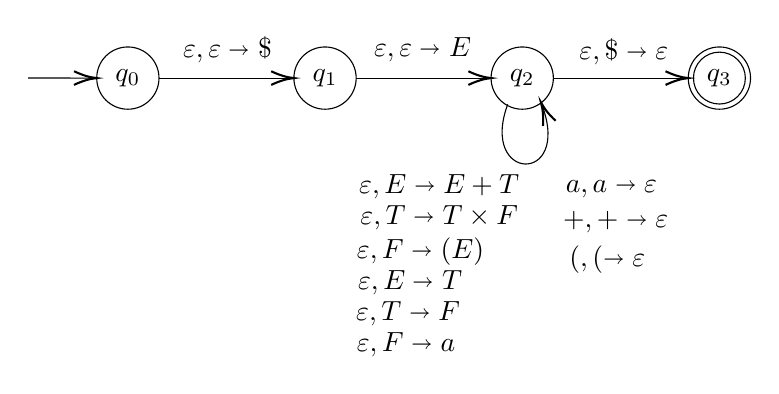
\begin{tikzpicture}[x=0.75pt,y=0.75pt,yscale=-1,xscale=1]
	%uncomment if require: \path (0,251.796875); %set diagram left start at 0, and has height of 251.796875
	
	%Shape: Circle [id:dp712656770325752] 
	\draw   (161,34.85) .. controls (161,26.56) and (167.72,19.85) .. (176,19.85) .. controls (184.28,19.85) and (191,26.56) .. (191,34.85) .. controls (191,43.13) and (184.28,49.85) .. (176,49.85) .. controls (167.72,49.85) and (161,43.13) .. (161,34.85) -- cycle ;
	%Shape: Circle [id:dp26800751361907005] 
	\draw   (448.5,34.85) .. controls (448.5,27.94) and (454.1,22.35) .. (461,22.35) .. controls (467.9,22.35) and (473.5,27.94) .. (473.5,34.85) .. controls (473.5,41.75) and (467.9,47.35) .. (461,47.35) .. controls (454.1,47.35) and (448.5,41.75) .. (448.5,34.85) -- cycle ;
	%Shape: Circle [id:dp3993497086973854] 
	\draw   (256,34.85) .. controls (256,26.56) and (262.72,19.85) .. (271,19.85) .. controls (279.28,19.85) and (286,26.56) .. (286,34.85) .. controls (286,43.13) and (279.28,49.85) .. (271,49.85) .. controls (262.72,49.85) and (256,43.13) .. (256,34.85) -- cycle ;
	%Straight Lines [id:da36406928281279294] 
	\draw    (128,34.8) -- (159,34.85) ;
	\draw [shift={(161,34.85)}, rotate = 180.09] [color={rgb, 255:red, 0; green, 0; blue, 0 }  ][line width=0.75]    (10.93,-3.29) .. controls (6.95,-1.4) and (3.31,-0.3) .. (0,0) .. controls (3.31,0.3) and (6.95,1.4) .. (10.93,3.29)   ;
	
	%Shape: Circle [id:dp21865328012254004] 
	\draw   (351,34.85) .. controls (351,26.56) and (357.72,19.85) .. (366,19.85) .. controls (374.28,19.85) and (381,26.56) .. (381,34.85) .. controls (381,43.13) and (374.28,49.85) .. (366,49.85) .. controls (357.72,49.85) and (351,43.13) .. (351,34.85) -- cycle ;
	%Straight Lines [id:da764690906183654] 
	\draw    (191,34.85) -- (254,34.85) ;
	\draw [shift={(256,34.85)}, rotate = 180] [color={rgb, 255:red, 0; green, 0; blue, 0 }  ][line width=0.75]    (10.93,-3.29) .. controls (6.95,-1.4) and (3.31,-0.3) .. (0,0) .. controls (3.31,0.3) and (6.95,1.4) .. (10.93,3.29)   ;
	
	%Straight Lines [id:da3140384669124394] 
	\draw    (286,34.85) -- (349,34.85) ;
	\draw [shift={(351,34.85)}, rotate = 180] [color={rgb, 255:red, 0; green, 0; blue, 0 }  ][line width=0.75]    (10.93,-3.29) .. controls (6.95,-1.4) and (3.31,-0.3) .. (0,0) .. controls (3.31,0.3) and (6.95,1.4) .. (10.93,3.29)   ;
	
	%Shape: Circle [id:dp7522514735889898] 
	\draw   (446,34.85) .. controls (446,26.56) and (452.72,19.85) .. (461,19.85) .. controls (469.28,19.85) and (476,26.56) .. (476,34.85) .. controls (476,43.13) and (469.28,49.85) .. (461,49.85) .. controls (452.72,49.85) and (446,43.13) .. (446,34.85) -- cycle ;
	%Straight Lines [id:da29212008129665823] 
	\draw    (381,34.85) -- (444,34.85) ;
	\draw [shift={(446,34.85)}, rotate = 180] [color={rgb, 255:red, 0; green, 0; blue, 0 }  ][line width=0.75]    (10.93,-3.29) .. controls (6.95,-1.4) and (3.31,-0.3) .. (0,0) .. controls (3.31,0.3) and (6.95,1.4) .. (10.93,3.29)   ;
	
	%Curve Lines [id:da5059282088478203] 
	\draw    (359,47.5) .. controls (345.21,84.93) and (389.63,86.46) .. (375.68,48.27) ;
	\draw [shift={(375,46.5)}, rotate = 428.2] [color={rgb, 255:red, 0; green, 0; blue, 0 }  ][line width=0.75]    (10.93,-3.29) .. controls (6.95,-1.4) and (3.31,-0.3) .. (0,0) .. controls (3.31,0.3) and (6.95,1.4) .. (10.93,3.29)   ;
	
	% Text Node
	\draw (176,34.85) node  [align=left] {$\displaystyle q_{0}$};
	% Text Node
	\draw (461,34.85) node  [align=left] {$\displaystyle q_{3}$};
	% Text Node
	\draw (271,34.85) node  [align=left] {$\displaystyle q_{1}$};
	% Text Node
	\draw (224,21.3) node  [align=left] {$\displaystyle \varepsilon ,\varepsilon \shortrightarrow \$$};
	% Text Node
	\draw (318,21.3) node  [align=left] {$\displaystyle \varepsilon ,\varepsilon \shortrightarrow E$};
	% Text Node
	\draw (326,87.3) node  [align=left] {$\displaystyle \varepsilon ,E\shortrightarrow E+T$};
	% Text Node
	\draw (312,133.3) node  [align=left] {$\displaystyle \varepsilon ,E\shortrightarrow T$};
	% Text Node
	\draw (326,102.3) node  [align=left] {$\displaystyle \varepsilon ,T\shortrightarrow T\times F$};
	% Text Node
	\draw (317,118.3) node  [align=left] {$\displaystyle \varepsilon ,F\shortrightarrow ( E)$};
	% Text Node
	\draw (311,148.3) node  [align=left] {$\displaystyle \varepsilon ,T\shortrightarrow F$};
	% Text Node
	\draw (310,163.3) node  [align=left] {$\displaystyle \varepsilon ,F\shortrightarrow a$};
	% Text Node
	\draw (409,88.3) node  [align=left] {$\displaystyle a,a\shortrightarrow \varepsilon $};
	% Text Node
	\draw (411,104.3) node  [align=left] {$\displaystyle +,+\shortrightarrow \varepsilon $};
	% Text Node
	\draw (407,122.3) node  [align=left] {$\displaystyle ( ,( \shortrightarrow \varepsilon $};
	% Text Node
	\draw (366,34.85) node  [align=left] {$\displaystyle q_{2}$};
	% Text Node
	\draw (415,22.3) node  [align=left] {$\displaystyle \varepsilon ,\$\shortrightarrow \varepsilon $};
	
	\end{tikzpicture}

\begin{problem}{2.12}
\end{problem}

	\tikzset{every picture/.style={line width=0.75pt}} %set default line width to 0.75pt        
	
	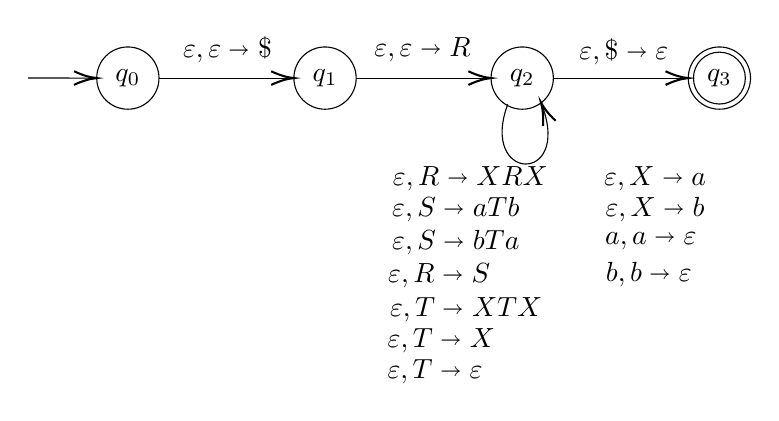
\begin{tikzpicture}[x=0.75pt,y=0.75pt,yscale=-1,xscale=1]
	%uncomment if require: \path (0,240.703125); %set diagram left start at 0, and has height of 240.703125
	
	%Shape: Circle [id:dp990920215192006] 
	\draw   (172,51.85) .. controls (172,43.56) and (178.72,36.85) .. (187,36.85) .. controls (195.28,36.85) and (202,43.56) .. (202,51.85) .. controls (202,60.13) and (195.28,66.85) .. (187,66.85) .. controls (178.72,66.85) and (172,60.13) .. (172,51.85) -- cycle ;
	%Shape: Circle [id:dp0904031948590649] 
	\draw   (459.5,51.85) .. controls (459.5,44.94) and (465.1,39.35) .. (472,39.35) .. controls (478.9,39.35) and (484.5,44.94) .. (484.5,51.85) .. controls (484.5,58.75) and (478.9,64.35) .. (472,64.35) .. controls (465.1,64.35) and (459.5,58.75) .. (459.5,51.85) -- cycle ;
	%Shape: Circle [id:dp1776071526101599] 
	\draw   (267,51.85) .. controls (267,43.56) and (273.72,36.85) .. (282,36.85) .. controls (290.28,36.85) and (297,43.56) .. (297,51.85) .. controls (297,60.13) and (290.28,66.85) .. (282,66.85) .. controls (273.72,66.85) and (267,60.13) .. (267,51.85) -- cycle ;
	%Straight Lines [id:da6779926529924325] 
	\draw    (139,51.8) -- (170,51.85) ;
	\draw [shift={(172,51.85)}, rotate = 180.09] [color={rgb, 255:red, 0; green, 0; blue, 0 }  ][line width=0.75]    (10.93,-3.29) .. controls (6.95,-1.4) and (3.31,-0.3) .. (0,0) .. controls (3.31,0.3) and (6.95,1.4) .. (10.93,3.29)   ;
	
	%Shape: Circle [id:dp6458826240842988] 
	\draw   (362,51.85) .. controls (362,43.56) and (368.72,36.85) .. (377,36.85) .. controls (385.28,36.85) and (392,43.56) .. (392,51.85) .. controls (392,60.13) and (385.28,66.85) .. (377,66.85) .. controls (368.72,66.85) and (362,60.13) .. (362,51.85) -- cycle ;
	%Straight Lines [id:da7693370339606864] 
	\draw    (202,51.85) -- (265,51.85) ;
	\draw [shift={(267,51.85)}, rotate = 180] [color={rgb, 255:red, 0; green, 0; blue, 0 }  ][line width=0.75]    (10.93,-3.29) .. controls (6.95,-1.4) and (3.31,-0.3) .. (0,0) .. controls (3.31,0.3) and (6.95,1.4) .. (10.93,3.29)   ;
	
	%Straight Lines [id:da3522744455936877] 
	\draw    (297,51.85) -- (360,51.85) ;
	\draw [shift={(362,51.85)}, rotate = 180] [color={rgb, 255:red, 0; green, 0; blue, 0 }  ][line width=0.75]    (10.93,-3.29) .. controls (6.95,-1.4) and (3.31,-0.3) .. (0,0) .. controls (3.31,0.3) and (6.95,1.4) .. (10.93,3.29)   ;
	
	%Shape: Circle [id:dp30631468478350987] 
	\draw   (457,51.85) .. controls (457,43.56) and (463.72,36.85) .. (472,36.85) .. controls (480.28,36.85) and (487,43.56) .. (487,51.85) .. controls (487,60.13) and (480.28,66.85) .. (472,66.85) .. controls (463.72,66.85) and (457,60.13) .. (457,51.85) -- cycle ;
	%Straight Lines [id:da09849739701009219] 
	\draw    (392,51.85) -- (455,51.85) ;
	\draw [shift={(457,51.85)}, rotate = 180] [color={rgb, 255:red, 0; green, 0; blue, 0 }  ][line width=0.75]    (10.93,-3.29) .. controls (6.95,-1.4) and (3.31,-0.3) .. (0,0) .. controls (3.31,0.3) and (6.95,1.4) .. (10.93,3.29)   ;
	
	%Curve Lines [id:da3472199513321359] 
	\draw    (370,64.5) .. controls (356.21,101.93) and (400.63,103.46) .. (386.68,65.27) ;
	\draw [shift={(386,63.5)}, rotate = 428.2] [color={rgb, 255:red, 0; green, 0; blue, 0 }  ][line width=0.75]    (10.93,-3.29) .. controls (6.95,-1.4) and (3.31,-0.3) .. (0,0) .. controls (3.31,0.3) and (6.95,1.4) .. (10.93,3.29)   ;
	
	% Text Node
	\draw (352,100.3) node  [align=left] {$\displaystyle \varepsilon ,R\shortrightarrow XRX$};
	% Text Node
	\draw (337,147.3) node  [align=left] {$\displaystyle \varepsilon ,R\shortrightarrow S$};
	% Text Node
	\draw (345,115.3) node  [align=left] {$\displaystyle \varepsilon ,S\shortrightarrow aTb$};
	% Text Node
	\draw (350,163.3) node  [align=left] {$\displaystyle \varepsilon ,T\shortrightarrow XTX$};
	% Text Node
	\draw (345,131.3) node  [align=left] {$\displaystyle \varepsilon ,S\shortrightarrow bTa$};
	% Text Node
	\draw (338,178.3) node  [align=left] {$\displaystyle \varepsilon ,T\shortrightarrow X$};
	% Text Node
	\draw (439,130.3) node  [align=left] {$\displaystyle a,a\shortrightarrow \varepsilon $};
	% Text Node
	\draw (438,146.3) node  [align=left] {$\displaystyle b,b\shortrightarrow \varepsilon $};
	% Text Node
	\draw (335,193.3) node  [align=left] {$\displaystyle \varepsilon ,T\shortrightarrow \varepsilon $};
	% Text Node
	\draw (441,100.3) node  [align=left] {$\displaystyle \varepsilon ,X\shortrightarrow a$};
	% Text Node
	\draw (441,115.3) node  [align=left] {$\displaystyle \varepsilon ,X\shortrightarrow b$};
	% Text Node
	\draw (187,51.85) node  [align=left] {$\displaystyle q_{0}$};
	% Text Node
	\draw (472,51.85) node  [align=left] {$\displaystyle q_{3}$};
	% Text Node
	\draw (282,51.85) node  [align=left] {$\displaystyle q_{1}$};
	% Text Node
	\draw (235,38.3) node  [align=left] {$\displaystyle \varepsilon ,\varepsilon \shortrightarrow \$$};
	% Text Node
	\draw (329,38.3) node  [align=left] {$\displaystyle \varepsilon ,\varepsilon \shortrightarrow R$};
	% Text Node
	\draw (377,51.85) node  [align=left] {$\displaystyle q_{2}$};
	% Text Node
	\draw (426,39.3) node  [align=left] {$\displaystyle \varepsilon ,\$\shortrightarrow \varepsilon $};
	
	\end{tikzpicture}

\begin{problem}{2.13}
\end{problem}
	\begin{enumerate}[label=(\alph*)]
	\item 
		There are two cases.	\\
		\hspace*{5mm} Case 1: N 0s and 2N 0s are separated by a \# where N is non negative integers.	\\
		\hspace*{5mm} Case 2: Three sets of 0s are separated by 2 \# where number of 0s in each set is any non negative integers. 
	\item 
		In case 1 mentioned above, number N need to be remembered to check if number of N in second set of 0s is correct. N can be infinite; therefore, the gammer is not regular. 
	\end{enumerate}

\begin{problem}{2.14}
\end{problem}
	$
	S \shortrightarrow BA_1 \: | \: BA \: | \: AB \: | \: 00 \: | \: \varepsilon	\\
	A \shortrightarrow BA_1 \: | \: BA \: | \: AB \: | \: 00	\\
	A_1 \shortrightarrow AB	\\
	B \shortrightarrow 00
	$

\begin{problem}{2.26}
\end{problem}
\hspace*{5mm} If $n=1$, steps required is 1 where $2 \times 1-1=1$ which is correct because single element takes one step to derive. Let $w_k$ be a string with k length and requires $2k-1$ steps to derive. Increase length of $w_k$ by 1 by functions $A \shortrightarrow BC$, $B \shortrightarrow b$ and $C \shortrightarrow c$. Steps required is also increased by 2. $w_{k+1}$ takes $2k-1+2=2k+1$ steps. According to the proving function, length of $w_{k+1}$ is $2(k+1)-1=2k+1$ which is same as the result above. \\ \\
\hspace*{5mm} According to mathematical induction, exactly $2n-1$ steps are required for any derivation of w where n is length of the string. 

\begin{problem}{2.30}
\end{problem}
\begin{enumerate}[label=(\alph*)]
	\item \addtocounter{enumi}{2}
		\hspace*{5mm} Assume the grammer is context free and let $p$ be pumping length. Consider $s=0^p1^p0^p1^p$ is a member of the grammer. By the pumping lemma, we can write $s$ as $uvxyz$. 	\\
		\hspace*{5mm} Suppose that v or y contains both 0s and 1s, order of 0s and 1s in string $uv^ixy^iz$ can not be correct. 	\\
		\hspace*{5mm} Suppose that v and y only contains single type of numbers, in string $uv^ixy^iz$, numbers each set of 0s and 1s cannot be the same.	

	\item
		\hspace*{5mm} Assume the grammer is context free and let $p$ be pumping length. Consider $s=a^pb^p\#a^pb^p$ is a member of the grammer. By the pumping lemma, we can write $s$ as $uvxyz$. 	\\
		\hspace*{5mm} Suppose x contains \#, in $uv^ixy^iz$, all a are in sequence after \#, but a are separated by bs before \#. Thus, x cannot contain \#. 	\\
		\hspace*{5mm} Suppose v or y contains \#, $uv^ixy^iz$ contains more than one \#, which is not member of s. 	\\
		\hspace*{5mm} Suppose u or z contains \#, v and y are at same side of \#, which means there are more symbols on one side of \#. In $a^pb^p\#a^pb^p$, there are same number of symbols in both side. u or z cannot contain \#. 

\end{enumerate}

\begin{problem}{2.31}
\end{problem}
	\hspace*{5mm} Assume the grammer is context free and let $p$ be pumping length. Consider $s=0^p1^{2p}0^p$ is a member of the grammer. By the pumping lemma, we can write $s$ as $uvxyz$. 	\\
	\hspace*{5mm} Suppose v and y only contain one type of number, in $uv^ixy^iz$, either number of 1s and 0s are not equal or number of left and right 0s are not the same. 	\\
	\hspace*{5mm} Suppose v or y contains both 0s and 1s, in $uv^ixy^iz$, order of numbers cannot be correct. Thus it is not member of s. 

\begin{problem}{2.32}
\end{problem}
	\hspace*{5mm} Assume the grammer is context free and let $p$ be pumping length. Consider $s=1^p3^q2^p4^q$ is a member of the grammer. By the pumping lemma, we can write $s$ as $uvxyz$, $|vxy| \leq p$ and $uv^ixy^iz$ is member of s. To keep number of 1s and 2s equal and number of 3s and 4s equal, v and y must contains 1 and 2 or 3 and 4 and so does $vxy$. Since $|vxy| \leq p$, $vxy$ can only contains 1,3 or 3,2 or 2,4. There is no way to have equal number of 1s and 2s and equal number of 3s and 4s in $uv^ixy^iz$. Therefore, such grammer is not context free. 	\\

\begin{problem}{2.47}
\end{problem}
\begin{enumerate}[label=(\alph*)]
	\item ~

		\tikzset{every picture/.style={line width=0.75pt}} %set default line width to 0.75pt        
		
		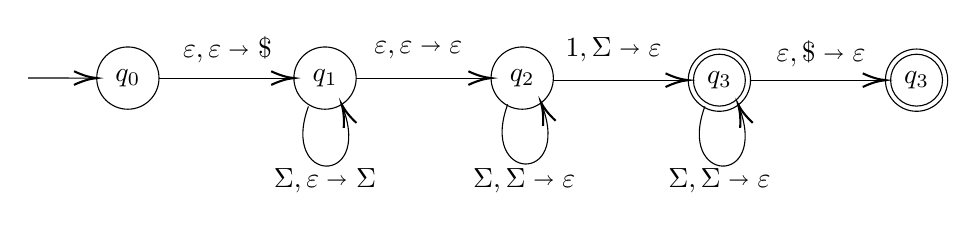
\begin{tikzpicture}[x=0.75pt,y=0.75pt,yscale=-1,xscale=1]
		%uncomment if require: \path (0,193.5); %set diagram left start at 0, and has height of 193.5
		
		%Shape: Circle [id:dp4821629125320397] 
		\draw   (135,57.85) .. controls (135,49.56) and (141.72,42.85) .. (150,42.85) .. controls (158.28,42.85) and (165,49.56) .. (165,57.85) .. controls (165,66.13) and (158.28,72.85) .. (150,72.85) .. controls (141.72,72.85) and (135,66.13) .. (135,57.85) -- cycle ;
		%Shape: Circle [id:dp4841331708650445] 
		\draw   (230,57.85) .. controls (230,49.56) and (236.72,42.85) .. (245,42.85) .. controls (253.28,42.85) and (260,49.56) .. (260,57.85) .. controls (260,66.13) and (253.28,72.85) .. (245,72.85) .. controls (236.72,72.85) and (230,66.13) .. (230,57.85) -- cycle ;
		%Straight Lines [id:da1761385414434613] 
		\draw    (102,57.8) -- (133,57.85) ;
		\draw [shift={(135,57.85)}, rotate = 180.09] [color={rgb, 255:red, 0; green, 0; blue, 0 }  ][line width=0.75]    (10.93,-3.29) .. controls (6.95,-1.4) and (3.31,-0.3) .. (0,0) .. controls (3.31,0.3) and (6.95,1.4) .. (10.93,3.29)   ;
		
		%Shape: Circle [id:dp8395032286912913] 
		\draw   (325,57.85) .. controls (325,49.56) and (331.72,42.85) .. (340,42.85) .. controls (348.28,42.85) and (355,49.56) .. (355,57.85) .. controls (355,66.13) and (348.28,72.85) .. (340,72.85) .. controls (331.72,72.85) and (325,66.13) .. (325,57.85) -- cycle ;
		%Straight Lines [id:da7537905252662744] 
		\draw    (165,57.85) -- (228,57.85) ;
		\draw [shift={(230,57.85)}, rotate = 180] [color={rgb, 255:red, 0; green, 0; blue, 0 }  ][line width=0.75]    (10.93,-3.29) .. controls (6.95,-1.4) and (3.31,-0.3) .. (0,0) .. controls (3.31,0.3) and (6.95,1.4) .. (10.93,3.29)   ;
		
		%Straight Lines [id:da30800310931321184] 
		\draw    (260,57.85) -- (323,57.85) ;
		\draw [shift={(325,57.85)}, rotate = 180] [color={rgb, 255:red, 0; green, 0; blue, 0 }  ][line width=0.75]    (10.93,-3.29) .. controls (6.95,-1.4) and (3.31,-0.3) .. (0,0) .. controls (3.31,0.3) and (6.95,1.4) .. (10.93,3.29)   ;
		
		%Curve Lines [id:da3438745542249422] 
		\draw    (333,70.5) .. controls (319.21,107.93) and (363.63,109.46) .. (349.68,71.27) ;
		\draw [shift={(349,69.5)}, rotate = 428.2] [color={rgb, 255:red, 0; green, 0; blue, 0 }  ][line width=0.75]    (10.93,-3.29) .. controls (6.95,-1.4) and (3.31,-0.3) .. (0,0) .. controls (3.31,0.3) and (6.95,1.4) .. (10.93,3.29)   ;
		
		%Curve Lines [id:da5969657367165231] 
		\draw    (237,71.5) .. controls (223.21,108.93) and (267.63,110.46) .. (253.68,72.27) ;
		\draw [shift={(253,70.5)}, rotate = 428.2] [color={rgb, 255:red, 0; green, 0; blue, 0 }  ][line width=0.75]    (10.93,-3.29) .. controls (6.95,-1.4) and (3.31,-0.3) .. (0,0) .. controls (3.31,0.3) and (6.95,1.4) .. (10.93,3.29)   ;
		
		%Shape: Circle [id:dp6409763567170343] 
		\draw   (517.5,58.85) .. controls (517.5,51.94) and (523.1,46.35) .. (530,46.35) .. controls (536.9,46.35) and (542.5,51.94) .. (542.5,58.85) .. controls (542.5,65.75) and (536.9,71.35) .. (530,71.35) .. controls (523.1,71.35) and (517.5,65.75) .. (517.5,58.85) -- cycle ;
		%Shape: Circle [id:dp9405598398536767] 
		\draw   (420,58.85) .. controls (420,50.56) and (426.72,43.85) .. (435,43.85) .. controls (443.28,43.85) and (450,50.56) .. (450,58.85) .. controls (450,67.13) and (443.28,73.85) .. (435,73.85) .. controls (426.72,73.85) and (420,67.13) .. (420,58.85) -- cycle ;
		%Straight Lines [id:da9795786953072845] 
		\draw    (355,58.85) -- (418,58.85) ;
		\draw [shift={(420,58.85)}, rotate = 180] [color={rgb, 255:red, 0; green, 0; blue, 0 }  ][line width=0.75]    (10.93,-3.29) .. controls (6.95,-1.4) and (3.31,-0.3) .. (0,0) .. controls (3.31,0.3) and (6.95,1.4) .. (10.93,3.29)   ;
		
		%Shape: Circle [id:dp9245607735304744] 
		\draw   (515,58.85) .. controls (515,50.56) and (521.72,43.85) .. (530,43.85) .. controls (538.28,43.85) and (545,50.56) .. (545,58.85) .. controls (545,67.13) and (538.28,73.85) .. (530,73.85) .. controls (521.72,73.85) and (515,67.13) .. (515,58.85) -- cycle ;
		%Straight Lines [id:da76211057110787] 
		\draw    (450,58.85) -- (513,58.85) ;
		\draw [shift={(515,58.85)}, rotate = 180] [color={rgb, 255:red, 0; green, 0; blue, 0 }  ][line width=0.75]    (10.93,-3.29) .. controls (6.95,-1.4) and (3.31,-0.3) .. (0,0) .. controls (3.31,0.3) and (6.95,1.4) .. (10.93,3.29)   ;
		
		%Curve Lines [id:da2745519177418694] 
		\draw    (428,71.5) .. controls (414.21,108.93) and (458.63,110.46) .. (444.68,72.27) ;
		\draw [shift={(444,70.5)}, rotate = 428.2] [color={rgb, 255:red, 0; green, 0; blue, 0 }  ][line width=0.75]    (10.93,-3.29) .. controls (6.95,-1.4) and (3.31,-0.3) .. (0,0) .. controls (3.31,0.3) and (6.95,1.4) .. (10.93,3.29)   ;
		
		%Shape: Circle [id:dp2578435872327296] 
		\draw   (422.5,58.85) .. controls (422.5,51.94) and (428.1,46.35) .. (435,46.35) .. controls (441.9,46.35) and (447.5,51.94) .. (447.5,58.85) .. controls (447.5,65.75) and (441.9,71.35) .. (435,71.35) .. controls (428.1,71.35) and (422.5,65.75) .. (422.5,58.85) -- cycle ;
		
		% Text Node
		\draw (245,107.3) node  [align=left] {$\displaystyle \Sigma ,\varepsilon \shortrightarrow \Sigma $};
		% Text Node
		\draw (290,44.3) node  [align=left] {$\displaystyle \varepsilon ,\varepsilon \shortrightarrow \varepsilon $};
		% Text Node
		\draw (341,107.3) node  [align=left] {$\displaystyle \Sigma ,\Sigma \shortrightarrow \varepsilon $};
		% Text Node
		\draw (435,107.3) node  [align=left] {$\displaystyle \Sigma ,\Sigma \shortrightarrow \varepsilon $};
		% Text Node
		\draw (384,44.3) node  [align=left] {$\displaystyle 1,\Sigma \shortrightarrow \varepsilon $};
		% Text Node
		\draw (150,57.85) node  [align=left] {$\displaystyle q_{0}$};
		% Text Node
		\draw (245,57.85) node  [align=left] {$\displaystyle q_{1}$};
		% Text Node
		\draw (198,44.3) node  [align=left] {$\displaystyle \varepsilon ,\varepsilon \shortrightarrow \$$};
		% Text Node
		\draw (340,57.85) node  [align=left] {$\displaystyle q_{2}$};
		% Text Node
		\draw (530,58.85) node  [align=left] {$\displaystyle q_{3}$};
		% Text Node
		\draw (435,58.85) node  [align=left] {$\displaystyle q_{3}$};
		% Text Node
		\draw (484,46.3) node  [align=left] {$\displaystyle \varepsilon ,\$\shortrightarrow \varepsilon $};
		
		\end{tikzpicture}

	\item
		$G$ = ($\{S,S_1,S_2\}, \{0,1\}, R, S$)	\\
		R is 	\\
			$S \to \Sigma S \Sigma \: | \: S_1$ 	\\
			$S_1 \to \Sigma S_2 1 \: | \: \Sigma 1$ 	\\
			$S_2 \to \Sigma S_2 \Sigma \: | \: \Sigma S_2 \: | \: \Sigma\Sigma \: | \: \Sigma$ 	\\

\end{enumerate}
\end{document}